\documentclass{article}
\usepackage[utf8]{inputenc}

\title{CSE 4471: Steganography Research Paper}
\author{Anish Anand, Aayush Bansal, Cade Santha, Jeffrey Valli}
\date{March 2021}

\usepackage{natbib}
\usepackage{graphicx}

\begin{document}

\maketitle

\section{Introduction}
There is a theory which states that if ever anyone discovers exactly what the Universe is for and why it is here, it will instantly disappear and be replaced by something even more bizarre and inexplicable.
There is another theory which states that this has already happened.

\section{Test}
This section is a test to see how Overleaf works.

\begin{figure}[h!]
\centering
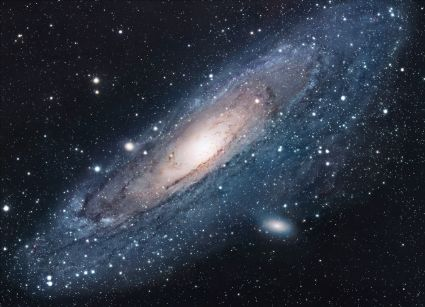
\includegraphics[scale=1.7]{universe}
\caption{The Universe}
\label{fig:universe}
\end{figure}

\section{Misdirection Steganography}
One flaw in the implementation of steganography can be evident when a third-party suspects that there is secret hidden data and other assets within a seemingly regular set of data. If the third-party is aware of common steganographic techniques, they may be able to easily uncover valuable assets guarded by steganography. In a work of research titled “Misdirection Steganography,” Takashi Mihara proposes the utilization of misdirection steganography to protect information assets from third-parties knowledgeable of secret data. In Mihara’s research paper, they bring forth the idea that misdirection steganography is an intersection of cryptography and steganographic techniques. In cryptography, the main goal is to prevent confidential secrets from getting into the hands of third parties. In steganography, the goal is to conceal the fact that certain information exists. 

Mihara’s proposed technique of misdirection steganography relies on the utilization of two kinds of secret data: true secret data and decoy secret data. The main goal of misdirection steganography would be to protect the true secret data by encouraging third parties to pay attention to the decoy secret data. The decoy secret data acts as a honeypot mechanism, preventing any further investigation into the existence of other secret data, as the third party is to believe that they found the secret data, but it is actually the decoy secret data.

The first step of formalizing misdirection steganography is to create a set of cover data and a true set of secret data. The secret data is stored as plain data to hide it from third parties. One downside to this is that it could be easily discovered and/or stolen if they are aware of its potential existence. In order to mitigate this, the next step is to utilize multi-level steganography through cryptography and compression. In this step, the secret plain data is encrypted and compressed and therefore replaced in the set. When implemented, the true secret data and the cover data are embedded at the relatively same position. It is possible to protect the true secret data by allowing the third party to discover the decoy data. It is recommended by Mihara to embed the secret data in the relatively same position within the decoy secret data, as the third party would not suspect any further data to be found. 

Mihara’s paper also includes the prospect of quantum misdirection steganography to further protect the secret data and references their other works for further exploration into the topic. By implementing misdirection steganography, the goals of concealing the existence of secret information as well protecting the information assets if a third-party suspects there is hidden data.

\section{Conclusion}
``I always thought something was fundamentally wrong with the universe'' \citep{adams1995hitchhiker}

\bibliographystyle{plain}
\bibliography{references}
\end{document}
